% !TeX spellcheck = it_IT
% !TEX encoding = utf8
\chapter{I Problemi del Millennio}
\begin{fullwidth}
	\begin{flushright}
		\emph{We must not believe those, who today, with philosophical bearing and deliberative tone, prophesy the fall of culture and accept the \emph{ignorabimus}. For us there is no \emph{ignorabimus}, and in my opinion none whatever in natural science. In opposition to the foolish \emph{ignorabimus} our slogan shall be: Wir m\"ussen wissen — wir werden wissen.('We must know - we will know.')% actually, questa cit starebbe meglio su un articolo su Hilbert oppure sul teorema di incompletezza di Godel
			}\\
		\vspace{0.5cm}
		\bfseries{David Hilbert}
	\end{flushright}
\end{fullwidth}

Nella vita di un matematico in erba sarà capitato almeno una volta di sentir parlare degli altisonanti “Problemi del Millennio”. Ebbene: Cosa sono? Perché periodicamente ritornano \emph{in auge}? Perché le soluzioni sono viste come il sacro Graal della matematica moderna? 

Cerchiamo innanzitutto di fare ordine spiegandone l’origine. Poi ci concentreremo su cosa sono e perché in tutto il mondo si venderebbe l’anima al diavolo per poterne risolvere uno (perlomeno l’autore di queste poche righe lo farebbe, pertanto mi scuso per essere stato così generalista \smiley).

\section{Hilbert “il complessato”}

8 agosto  1900. Parigi. Il mondo è in fermento. La famosa Esposizione di Parigi era in corso. La torre dell’ingegnere Eiffel era stata completata da pochi mesi. Tuttavia la storia sta per ricordare quel giorno per un altro motivo: David Hilbert, visto già allora come una leggenda vivente, annuncia al “Congresso internazionale dei matematici” i suoi 23 problemi. La storia stava per cambiare. 

\begin{marginfigure}%
	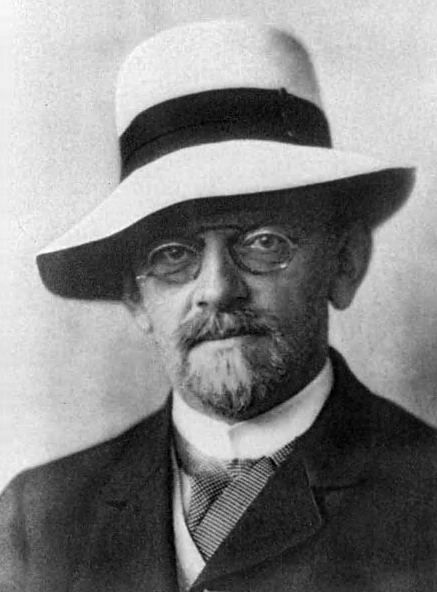
\includegraphics[width=\linewidth]{Hilbert}
	\caption{David Hilbert}
	\label{fig:Hilbert}
\end{marginfigure}

I problemi, per ammissione stessa di Hilbert, non erano i problemi al tempo più difficili da risolvere ma erano delle questioni aperte la cui risoluzione si sarebbe rivelata fondamentale per lo sviluppo della società e delle scienze in generale. Essi spaziavano dall’algebra, all’analisi e al calcolo delle variazioni, alla teoria dei numeri fino alla fisica teorica intesa in senso moderno.

Originariamente i problemi non erano 23; Hilbert ne enunciò solo 10, gli altri arrivarono 2 anni dopo, nel 1902. Oggi molti problemi sono stati risolti (le medaglie Fields sono fioccate grazie alla risoluzione di anche uno solo di questi problemi), altre risposte sono ancora in fase di validazione, altri problemi sono ora considerati “non-ben posti” in quanto troppo vaghi o comunque non abbastanza precisi mentre solo due sono considerati ancora “problemi aperti”.
\begin{marginfigure}%
	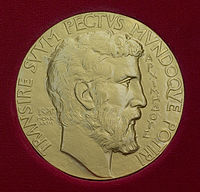
\includegraphics[width=\linewidth]{MedFields}
	\caption{La celeberrima Medaglia Fields: il "premio Nobel" della matematica.Sul Recto vie è inciso il volto di Archimede e la sua frase: \emph{Transire suum pectus mundoque potiri}(Elevarsi al di sopra di se stessi e conquistare il mondo).}
	\label{fig:fields}
\end{marginfigure}
\section{Filantropia portami via}

Nel 1998 l’impreditore milionario filantropo Landon T. Clay fonda con sua moglie e con il matematico Arthur Jaffe in una piccola cittadina del Massachusetts quello cha da li a poco sarebbe diventato l’Istituto matematico Clay (Clay Mathematics Institute o CMI). L’intento era di creare un ente privato \emph{no-profit} dedicata all'accrescimento ed alla diffusione della conoscenza della matematica.

Ad oggi l’associazione è famosa soprattutto per il Millenum Prize Problems ma si occupa a tutti gli effetti di volontariato \emph{tot court}: ogni anno borse di studio vengono erogate per studenti promettenti, summer schools vengono organizzate e sostenute nonché convegni, conferenze pubbliche e attività di pubblicizzazione della matematica rivolte soprattutto ai giovani, dal livello dei diplomati fino a quello dei ricercatori.

\section{I modesti “Problemi del Millennio”}

Il 24 maggio 2000, durante il Convegno del Millennio a Parigi (del resto non poteva non essere a Parigi e non chiamarsi così \smiley),  sulla falsa riga dell’idea di Hilbert di un secolo prima, l’istituto Clay pubblica una lista di 7 problemi ancora irrisolti. Allo stesso tempo viene pubblicata anche la procedura con la quale le eventuali soluzioni saranno verificate, nonché il premio che l’istituto offrirà al primo che avanzerà una soluzione accettabile di almeno un problema: l’esorbitante cifra di un \textbf{milione di Dollari} (come se la gloria eterna non fosse già abbastanza).

Come nell’idea originale di Hilbert, questi non sono né i più difficili da dimostrare computazionalmente, né i problemi con le dimostrazioni più difficili: sono solo una lista di problemi \emph{estremamente} importanti. Va notato inoltre come la lista proposta dal Clay Institute sia tutt’altro che esaustiva! Tuttavia molte soluzioni di problemi quantomai attuali possono essere corroborate o smentite grazie agli strumenti matematici che la soluzione a uno dei problemi del millennio può fornire (si veda per esempio alcune possibili soluzioni alla gravitazione quantistica o della rinomata Teoria delle Stringhe). 

Attualmente solo uno ne è stato risolto (dunque i milioni a disposizione, se la matematica non è un’opinione, e non lo è, sono ancora 6) e rispetto alla lista originale di Hilbert ne ricompare solo uno e probabilmente il più famoso...

Vediamo dunque quali sono questi famigerati problemi! Ne darò solo un assaggio (un libro intero non potrebbe bastare solo per uno solo, figuriamoci per tutti e 7 ;) ) e mi soffermerò in particolar modo su quelli che mi hanno toccato in prima persona in una maniera o nell’altra:

\subsection{1.Congettura di Poincaré}
Il problema è a cavallo tra la Topologia e la Geometria Differenziale\sidenote{Unico problema attualmente risolto}. 
È stato risolto nel 2003 grazie soprattutto al contributo del ninja della matematica, il russo Grigori Perelman e grazie a questo è uno dei matematici più famosi al mondo.
\begin{marginfigure}%
	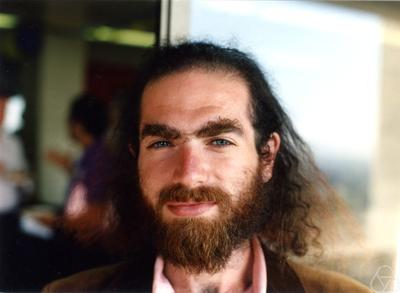
\includegraphics[width=\linewidth]{Perelman}
	\caption{Grigorij Jakovlevi\v{c} Perel'man%non rieco a scriverlo in russo!
		%(in russo: Григорий Яковлевич Перельман
		; Leningrado, 13 giugno 1966)}
	\label{fig:perelman}
\end{marginfigure}
Dopo che gli venne riconosciuta la paternalità del risultato, si tentò subito di fargli recapitare  il premio a 6 zeri. Perelman con \emph{nonchalance} rifiutò. E fin qui uno può dire: ”Ok”. Nel mentre si procedette a proclamarlo vincitore della medaglia Fields. Perelman, testardamente, rifiutò anche quella. Ok. La sua motivazione è stata ”il mio contibuto non è stato poi così importante”. Ok. Adesso vive con la madre nella periferia di San Pietroburgo. \emph{De gustibus} verrebbe da dire… della serie: \emph{fate vobis}.
\subsection{2.P versus NP} 
Immaginate di essere al ristorante\sidenote{probabilmente verrà risolto nei prossimi 50 anni}; davanti a voi avete un menù lungo 10 pagine. Vi viene chiesto di dire tutte le possibile combinazioni di piatti, in ogni quantità vogliate, la cui somma dia, diciamo, 46,00€. Questo problema può essere facilmente reso più difficile aggiungendo magari qualche costrizione, come per esempio “bisogna prendere almeno una porzione di Strudel della nonna di Erik” (una volta assunto che sia nel menù ;) ). Bene, ma non benissimo. Questo è il \emph{Knapsack Problem} (problema dello zaino).Questi tipi di problemi sono detti \emph{NP-completi}. Ovviamente è molto facile verificare se una soluzione è valida; totalmente diverso è trovarla! [foto da https://xkcd.com/287/]. Adesso la questione è: problemi che hanno la verifica semplice di un’ipotetica soluzione, hanno anche almeno un algoritmo semplice per trovarla? Innanzitutto bisogna capire cosa vuol dire \emph{semplice}… per comodità diciamo che un algoritmo semplice è uno che ci mette al più un tempo polinomiale per terminare (P appunto). Se così non è, sarà Non-Polinomiale (NP).  Molti sono convinti che P non sia equivalente a NP, ma attualmente nessuno sa la risposta. Se per caso un giorno si mostrerà che P=NP, beh vi consiglio di correre in banca a ritirare i vostri soldi prima e cancellarvi da Facebook poi. Le vostre passwords non serviranno più a nulla.
\subsection{3.Esistenza e regolarità delle soluzioni delle equazioni di Navier-Stokes}
Il problema è forse il più attuale in fisica matematica e nel campo dell’Analisi Reale. 
	
Le equazioni (meglio, sistema di equazioni) descrivono il moto di un fluido in regime turbolento. Sappiamo già risolvere le equazioni nel caso laminare (il caso per esempio dell’aria che passa sul parabrezza della vostra macchina quando siete in movimento), ma il caso turbolento è tutto un altro paio di maniche.
Per completezza scrivo di seguito la famosa equazione nel caso di un fluido \emph{compressibile}\sidenote{l'aria per esempio lo è, l'acqua no} 
\[\rho \left(\frac{\partial u }{\partial t}+u\cdot \nabla u\right)=-\nabla p+\nabla\cdot (\mu(\nabla u+(\nabla u)^{T})-\frac{2}{3}\mu(\nabla\cdot u)I)+F  \]
[foto: sinistra laminare, destra turbolento]\sidenote{dove $ u$ indica la velocità del fluido, $ p$ è la pressione del fluido, $ \mu$ è la viscosità dinamica del fluido e $ \rho$ è la densità del fluido.}
\subsection{4.Congettura di Riemann}
\label{par:Riemann}
Un classico. Famosissimo e rinomatissimo. Esso fa parte sia dell’analisi complessa sia della toria dei numeri. Tutto si basa sulla funzione $ \zeta$ (si legge zeta) di Riemann(-Eulero). La funzione, scoperta da Eulero e poi estesa da Riemann, è la seguente 
\[ \zeta(s)=\sum_{n=1}^{\infty} \frac{1}{n^s}\]
dove $ s=\sigma + i t$ è un numero complesso. È già dimostrato che la serie converge (cioè la somma non va a $ +\infty$, che è un bene) per $ sigma>1$. L’ipotesi di Riemann dice che gli zeri \emph{non-banali} di questa funzione si distribuiscono sulla retta complessa $ \sigma = 1/2$.
Ci si potrebbe benissimo chiedere perché questa funzione sia così importante… Ebbene, verificare se un numero è primo oppure no richiede un sacco di tempo. Per esempio 31, 331, 3331, 33331, 333331, 3333331, 33333331 sono tutti primi. Ma per qualche stramaledetta ragione, 333333331 non lo è!! Risolvere la congettura di Riemann ci potrebbe dare uno strumento potentissimo per la risoluzione di problemi di questo tipo.

\subsection{5.Esistenza di Yang–Mills e differenza di massa}
Siamo di nuovo nella Fisica-Matematica, questa volta nella teoria quantistica dei campi.

Chiariamo la situazione; la Teoria di Yang-Mills è un insieme di equazioni che predicono il comportamento di un sistema di particelle all’interno di un campo quantistico. Un campo quantistico a sua volta è una struttura matematica che segue un certo numero di regole.  
Bene. Questo problema richiede una dimostrazione che Young e Mills hanno fatto solo per spazi euclidei di dimensione 4 e può predire in modo corretto il comportamento di particelle di massa maggiore di zero(cioè tutte quelle con cui abbiamo a che fare tutti i giorni, ma non i fotoni tanto per capirci). Questa dimostrazione tuttavia non è basata su una teoria matematica solida, sebbene il risultato sia probabilmente vera (ad oggi non ci sono evidenze sperimentali che la contraddicano). La riformulazione della soluzione porterà probabilmente alla nascita di una nuova matematica. 

\subsection{6.Congettura di Hodge}
Topologia alebrica e Geometria Algebrica. Eh? Niente paura, tanti si spaventano… L’origine della geometria è insita nel procedimento di prendere oggetti (anche astratti) semplici e farne delle combinazioni per renderli più complicati. La congettura di Hodge dice che per un particolare tipo di spazio, chiamato \emph{spazio algebrico proiettivo}, gli spazi che lo compongono sono combinazioni lineari di strutture geometriche.
La difficoltà nel riuscire a dimostrarlo risiede anche nella difficoltà a comprenderlo. Ancora non è stato compreso a fondo e probabilmente la sua soluzione richiederà molta matematica “nuova”.

\subsection{7.Congettura di Birch e Swinnerton-Dyer }
Teoria dei numeri – Questo problema è il più difficile di quelli enunciati. Potrebbe non essere mai risolto.

Esso è a proposito dell’equazione diofantea preferita da tutti\sidenote{le equazioni diofanteee, che prendono il nome da Diofanto, sono equazioni algebriche la cui particolarità è che le soluzioni devono essere numeri interi}, cioè
\[ x^2+y^2=z^2\]
Euclide ha risolto questo problema per la dimensione 2. Per curve più complicate questo diviene più difficile e sopratutto non ci sono metodi genrali per risolverlo! Questa affascinante congettura dice che la dimensione del gruppo dei numeri razionali che risolvono l’equazione è in qualche modo legata alla Funzione Zeta di Riemann (sempre Lei!)\sidenote{vedi il paragrafo a pagina \pageref{par:Riemann}} valutata in quel punto! Cioè se è zero, ci sono infiniti punti razionali che la soddisfano, altrimenti sono finiti.

\section{Ok ho la soluzione di un problema. Ora cosa faccio?}
Eh? Innanzitutto vi dico che questo sito non fa più per voi ;). In ogni caso, \emph{for the sake of completeness}, dovete procedere in questo modo:






